\section{Representation and Description\buch{Ch. 11}\buchSeite{796-860}}
\label{sec:representationDescription}
\subsection{Representation\buchSeite{796}}
After the image segmentation, the boundaries need to be represented in a form, that is suitable for further processing.
\subsubsection{Boundary following\buchSeite{796}}
The following algorithm is the moore boundary tracking algorithm.
\begin{enumerate}
\item Let the starting point, $b_0$ be the uppermost, leftmost point in the image that is labeled 1. Denote by $c_0$ the west neighbor of $b_0$ clearly, $c_0$ is a background point. Examine the 8-neighbors of $b_0$, starting at $c_0$ and procedding in a clockwise direction. Let $b_1$ denote the first neighor encountered whose value is 1, and let $c_1$ be the (background) point immediately preceding $b_1$ in the sequence. Store the localtions of $b_0$ and $b_1$ for use in Step 5.
\item Let $b=b_1$ and $c=c_1$
\item Let the 8-neighbors of $b$, starting at $c$ and proceeding in a clockwise direction, be denoted by $n_1,n_2,\ldots,n_8$. Find the first $n_k$ labeled 1.
\item Let $b=n_k$ and $c=n_{k-1}$
\item Repeat Steps 3 and 4 until $b=b_0$ and the next boundary point found is $b_1$. The sequence of $b$ points found when the algorithm stops constitutes the set of ordered boundary points
\end{enumerate}
\begin{figure}[h]
	\centering
	\begin{subfigure}[b]{0.19\textwidth}
		\centering
		\adjustbox{scale=0.5}{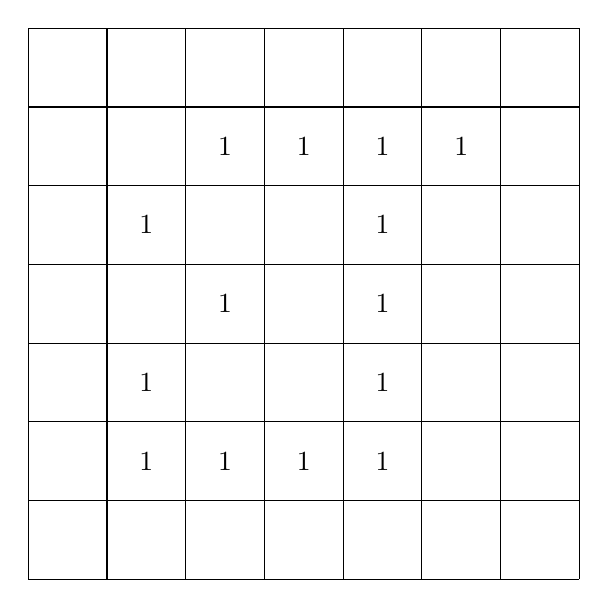
\begin{tikzpicture}

\foreach \x in {0,...,7} {
	\draw (\x,0) -- (\x,7);
	\draw (0,\x) -- (7,\x);
}

\foreach \x/\y in {1/1,1/2,2/3,1/4,2/5,3/5,4/5,5/5,4/4,4/3,4/2,4/1,3/1,2/1} {
	\node at  (\x+0.5,\y+0.5) {1};
}

\end{tikzpicture}}
		\caption{Step 1}
	\end{subfigure}
	\begin{subfigure}[b]{0.19\textwidth}
		\centering
		\adjustbox{scale=0.5}{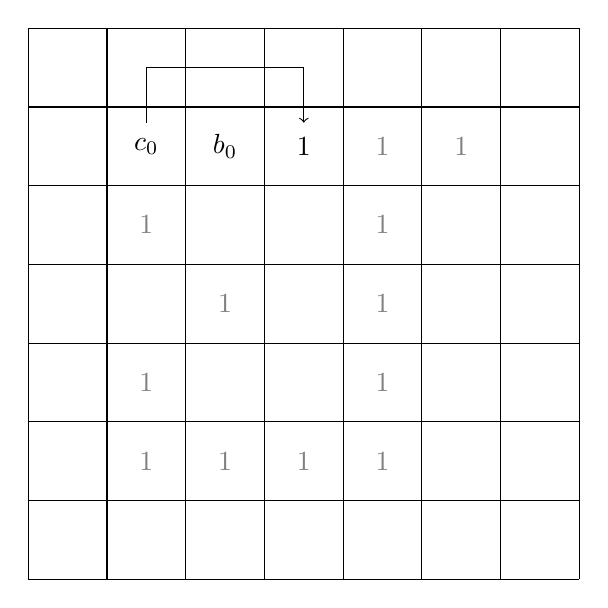
\begin{tikzpicture}

\foreach \x in {0,...,7} {
	\draw (\x,0) -- (\x,7);
	\draw (0,\x) -- (7,\x);
}

\node at (1.5,5.5) {$c_0$};
\node at (2.5,5.5) {$b_0$};
\node at (3.5,5.5) {1};
\foreach \x/\y in {1/1,1/2,2/3,1/4,4/5,5/5,4/4,4/3,4/2,4/1,3/1,2/1} {
	\node [gray] at  (\x+0.5,\y+0.5) {1};
}
\draw [->] (1.5,5.8) -- (1.5,6.5) -- (3.5,6.5) -- (3.5,5.8);

\end{tikzpicture}}
		\caption{Step 2}
	\end{subfigure}
	\begin{subfigure}[b]{0.19\textwidth}
		\centering
		\adjustbox{scale=0.5}{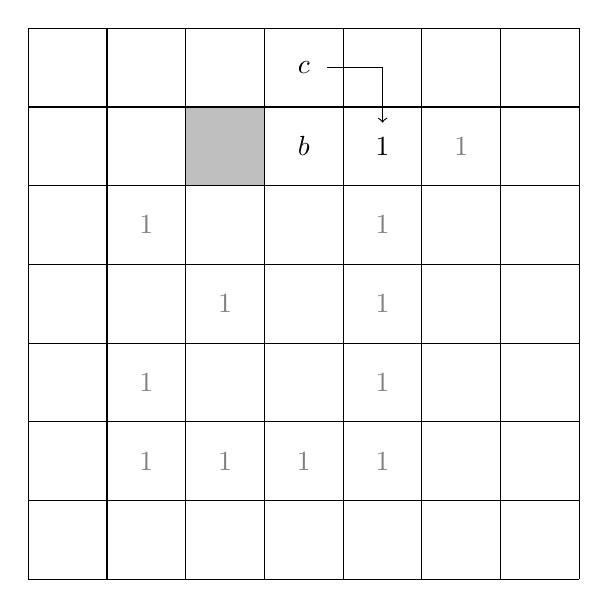
\begin{tikzpicture}

\foreach \x in {0,...,7} {
	\draw (\x,0) -- (\x,7);
	\draw (0,\x) -- (7,\x);
}

\draw[fill=lightgray] (2,5) rectangle (3,6);
\node at (3.5,6.5) {$c$};
\node at (3.5,5.5) {$b$};
\node at (4.5,5.5) {1};
\foreach \x/\y in {1/1,1/2,2/3,1/4,5/5,4/4,4/3,4/2,4/1,3/1,2/1} {
	\node [gray] at  (\x+0.5,\y+0.5) {1};
}
\draw [->] (3.8,6.5) -- (4.5,6.5) -- (4.5,5.8);

\end{tikzpicture}}
		\caption{Step 3}
	\end{subfigure}
	\begin{subfigure}[b]{0.19\textwidth}
		\centering
		\adjustbox{scale=0.5}{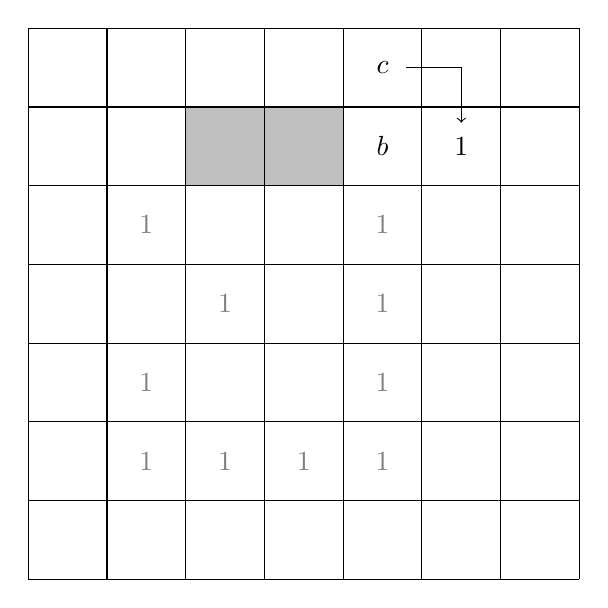
\begin{tikzpicture}

\foreach \x in {0,...,7} {
	\draw (\x,0) -- (\x,7);
	\draw (0,\x) -- (7,\x);
}

\draw[fill=lightgray] (2,5) rectangle (3,6);
\draw[fill=lightgray] (3,5) rectangle (4,6);
\node at (4.5,6.5) {$c$};
\node at (4.5,5.5) {$b$};
\node at (5.5,5.5) {1};
\foreach \x/\y in {1/1,1/2,2/3,1/4,4/4,4/3,4/2,4/1,3/1,2/1} {
	\node [gray] at  (\x+0.5,\y+0.5) {1};
}
\draw [->] (4.8,6.5) -- (5.5,6.5) -- (5.5,5.8);

\end{tikzpicture}}
		\caption{Step 4}
	\end{subfigure}
	\begin{subfigure}[b]{0.19\textwidth}
		\centering
		\adjustbox{scale=0.5}{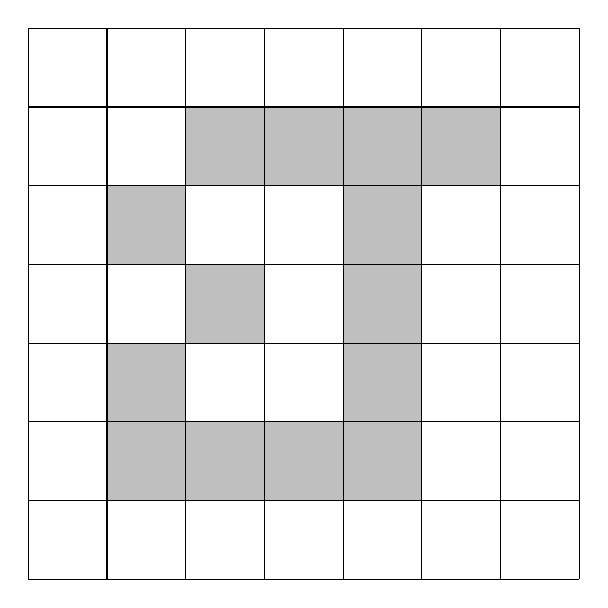
\begin{tikzpicture}

\foreach \x in {0,...,7} {
	\draw (\x,0) -- (\x,7);
	\draw (0,\x) -- (7,\x);
}

\foreach \x/\y in {1/1,1/2,2/3,1/4,2/5,3/5,4/5,5/5,4/4,4/3,4/2,4/1,3/1,2/1} {
	\draw [fill=lightgray] (\x,\y) rectangle (\x+1,\y+1);
}

\end{tikzpicture}}
		\caption{Result}
	\end{subfigure}
	\caption{Boundary Following Algorithm}
\end{figure}
Of course this algorithm also works counter-clock-wise.

\subsubsection{Chain codes\buchSeite{798}}
Chain codes are used to represent a boundary by a connected sequence of straight-line segments of specified length and direction. The direction of each segment is coded using a number.
\begin{figure}[h]
	\centering
	\begin{subfigure}[b]{0.3\textwidth}
		\centering
		\adjustbox{scale=1}{\begin{tikzpicture}

\foreach [count=\i] \x/\y in {1/0, 0/1, -1/0, 0/-1} {
	\draw [->, shorten >= 6, shorten <= 2] (0,0) -- (\x,\y) node {\i};
}

\end{tikzpicture}}
		\caption{4-directional}
	\end{subfigure}
	\begin{subfigure}[b]{0.3\textwidth}
		\centering
		\adjustbox{scale=1}{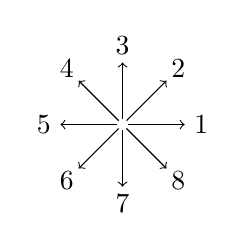
\begin{tikzpicture}
\pgfmathsetmacro{\a}{sin(45)}

\foreach [count=\i] \x/\y in {1/0, \a/\a, 0/1, -\a/\a, -1/0, -\a/-\a, 0/-1, \a/-\a } {
	\draw [->, shorten >= 6, shorten <= 2] (0,0) -- (\x,\y) node {\i};
}

\end{tikzpicture}}
		\caption{8-directional}
	\end{subfigure}
	\begin{subfigure}[b]{0.3\textwidth}
		\centering
		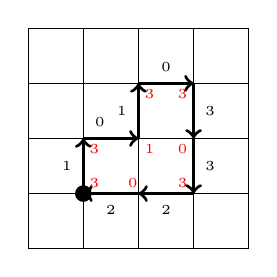
\begin{tikzpicture}[scale=0.7]
	% Grid
	\foreach \x in {0,1,2,3,4} {
	\draw (\x,0) -- (\x,4);
	\draw (0,\x) -- (4,\x);}
	
	% starting point and arrows
	\node[circle,fill=black,inner sep=0pt,minimum size=6pt] at (1,1) {};
	\draw[very thick,->] (1,1) -- (1,2);
	\draw[very thick,->] (1,2) -- (2,2);
	\draw[very thick,->] (2,2) -- (2,3);
	\draw[very thick,->] (2,3) -- (3,3);
	\draw[very thick,->] (3,3) -- (3,2);
	\draw[very thick,->] (3,2) -- (3,1);
	\draw[very thick,->] (3,1) -- (2,1);
	\draw[very thick,->] (2,1) -- (1,1);
	
	% chain codes
	\node at (0.7,1.5) {\tiny 1};
	\node at (1.3,2.3) {\tiny 0};
	\node at (1.7,2.5) {\tiny 1};
	\node at (2.5,3.3) {\tiny 0};
	\node at (3.3,2.5) {\tiny 3};
	\node at (3.3,1.5) {\tiny 3};
	\node at (2.5,0.7) {\tiny 2};
	\node at (1.5,0.7) {\tiny 2};
	
	% first order difference
	\node[color=red] at (1.2,1.2) {\tiny 3};
	\node[color=red] at (1.2,1.8) {\tiny 3};
	\node[color=red] at (2.2,1.8) {\tiny 1};
	\node[color=red] at (2.2,2.8) {\tiny 3};
	\node[color=red] at (2.8,2.8) {\tiny 3};
	\node[color=red] at (2.8,1.8) {\tiny 0};
	\node[color=red] at (2.8,1.2) {\tiny 3};
	\node[color=red] at (1.9,1.2) {\tiny 0};
	
\end{tikzpicture}
		\caption{Example}
		\label{fig:chaincode_example}
	\end{subfigure}
	\caption{Direction numbers for chain codes}
\end{figure}

Cain codes are quite sensitive to small disturbances. If they are on the pixel grid, they tend to result in rather long codes. Subsampling the boundary, i.e. going to a coarser grid results in a more robust and more efficient code at the expense of representation accuracy.\\
The resulting code depends on the starting point, which is not desirable. An easy trick is to circumvent this, is the convention to start at that point wich will result in a chain code that represents the smalles integer.\\

The representation can be made independent of rotation by using the \emph{first difference}. 
For each segment, assume the current direction is 0 and encode the direction of the next segment as before. \\
Example: Fig. \ref{fig:chaincode_example}. black: chain code, red: first difference.

\subsubsection{Polygonal approximation using Minimum perimeter polygon MPP\buchSeite{801}}
A boundary is represented by a polygon. The goal is to use as few segments as possible, while still capturing the essential features of the boundary. There exist simple approximations which in practice are often good enough\\
\paragraph{Minimum perimeter polygon MPP}
\begin{figure}[h]
	\centering
	\begin{subfigure}[b]{0.3\textwidth}
		\centering
		\adjustbox{scale=0.4}{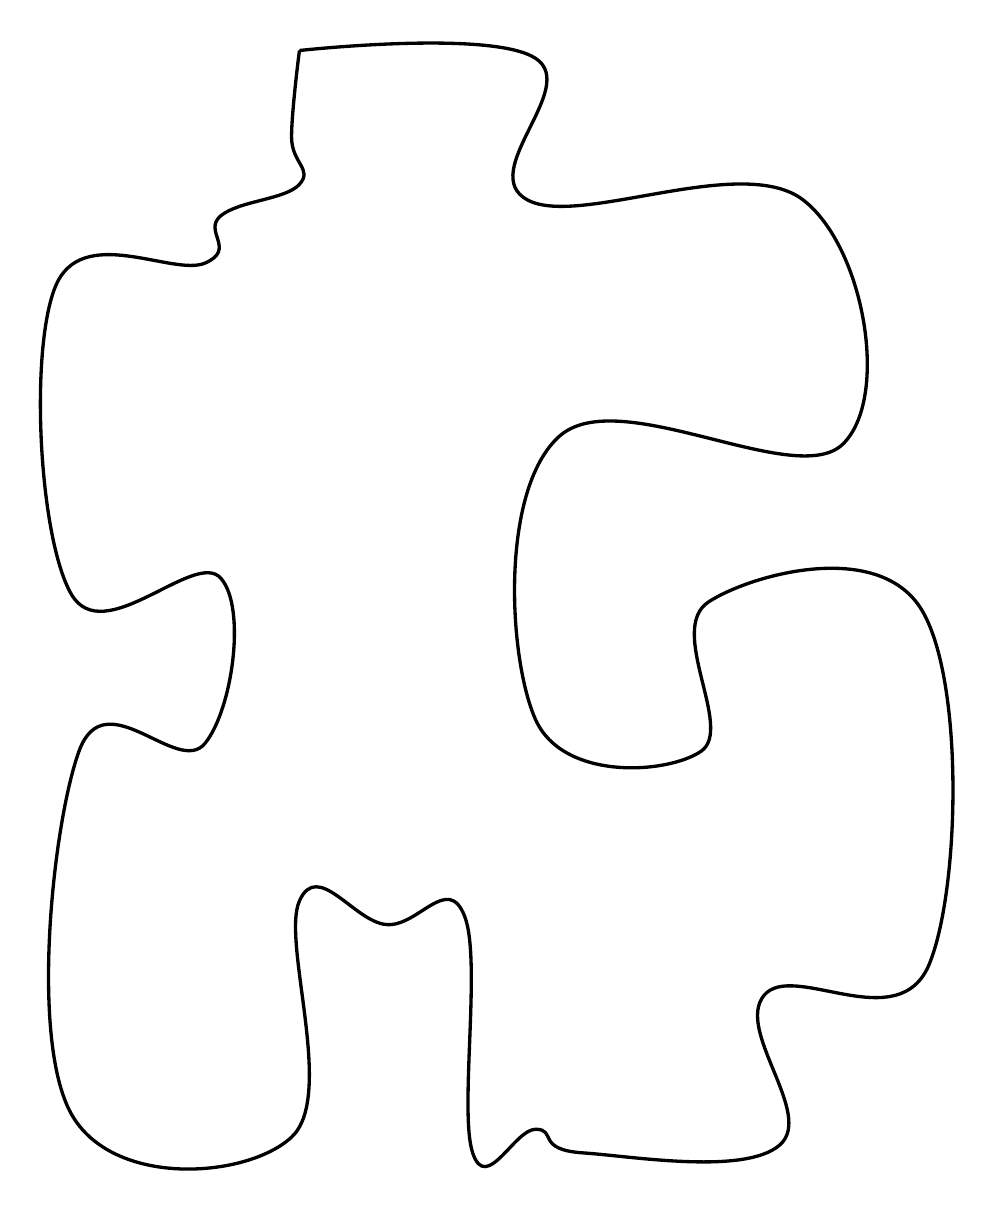
\begin{tikzpicture}
  
 \draw [very thick] plot[smooth, tension=.7] coordinates {(3.5,14.4) (6.5,14.3) (6.4,12.5) (9.9,12.5) (10.4,9.4) (6.8,9.5) (6.5,5.9) (8.6,5.5) (8.7,7.4) (11.4,7.3) (11.5,2.8) (9.4,2.4) (9.6,0.5) (7.1,0.4) (6.5,0.7) (5.7,0.4) (5.6,3.4) (4.6,3.3) (3.5,3.6) (3.4,0.6) (0.6,0.9) (0.7,5.5) (2.3,5.6) (2.5,7.7) (0.6,7.5) (0.4,11.4) (2.3,11.7) (2.5,12.3) (3.5,12.7) (3.4,13.3) (3.5,14.4)};

\end{tikzpicture}}
		\caption{Object Boundary}
	\end{subfigure}
	\begin{subfigure}[b]{0.3\textwidth}
		\centering
		\adjustbox{scale=0.4}{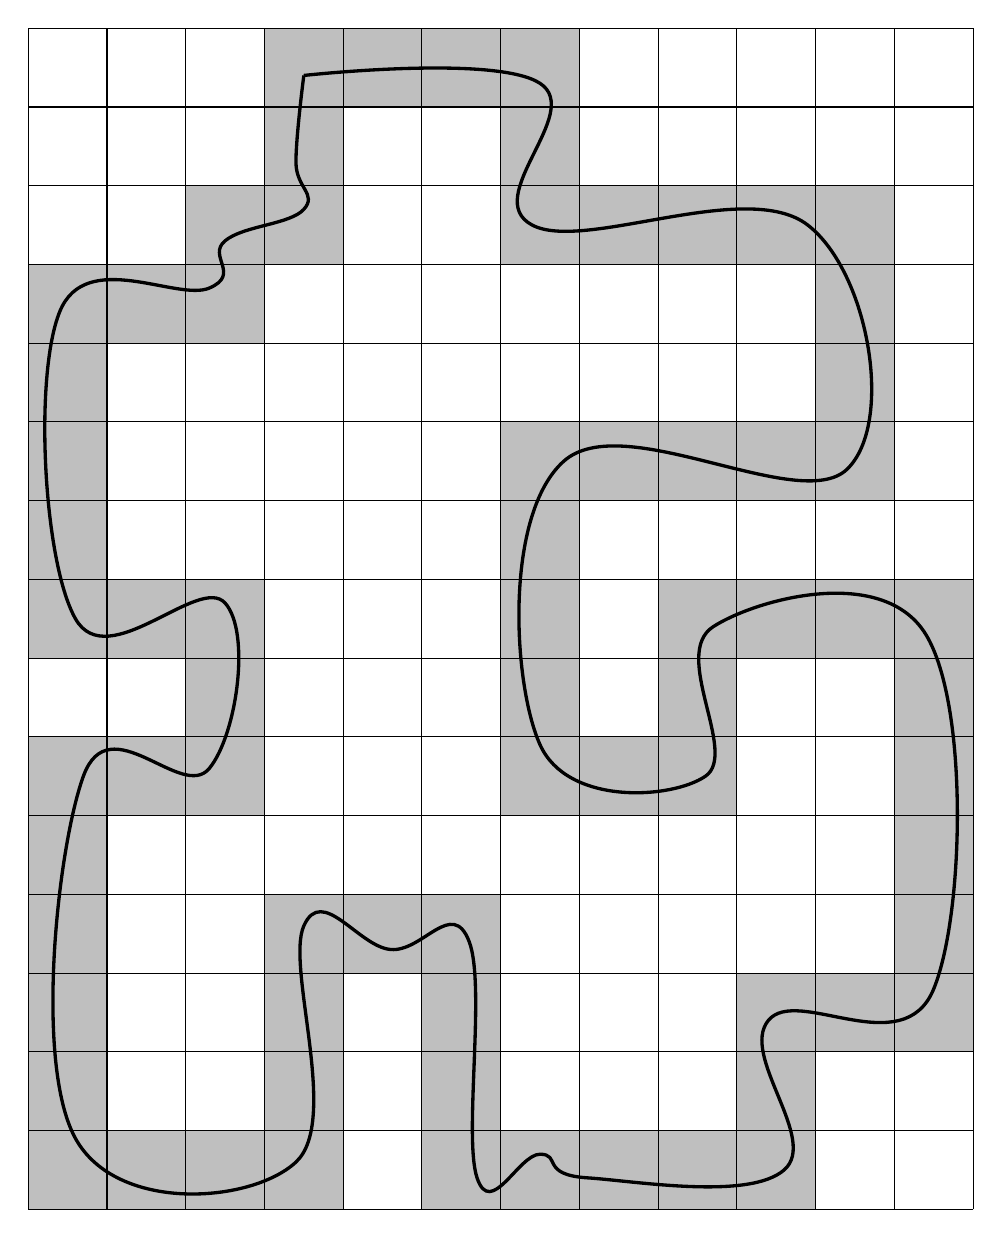
\begin{tikzpicture}

\draw [fill=lightgray] (0,12) rectangle (1,7)
 (1,8) rectangle (3,7)
  (3,5) rectangle (2,7)
  (2,5) rectangle (0,6)
  (0,5) rectangle (1,0)
  (1,0) rectangle (4,1)
  (4,1) rectangle (3,4)
  (4,4) rectangle (6,3)
  (5,3) rectangle (6,0)
  (6,0) rectangle (10,1)
  (10,1) rectangle (9,3)
  (10,3) rectangle (12,2)
  (12,3) rectangle (11,8)
  (11,8) rectangle (8,7)
  (8,7) rectangle (9,5)
  (8,5) rectangle (6,6)
  (7,6) rectangle (6,10)
  (7,10) rectangle (11,9)
 (11,10) rectangle (10,13)
  (10,13) rectangle (6,12)
  (7,13) rectangle (6,15)
  (6,15) rectangle (3,14)
  (3,14) rectangle (4,12)
  (2,13) rectangle (3,11)
  (2,12) rectangle (1,11);
  
 \draw [very thick] plot[smooth, tension=.7] coordinates {(3.5,14.4) (6.5,14.3) (6.4,12.5) (9.9,12.5) (10.4,9.4) (6.8,9.5) (6.5,5.9) (8.6,5.5) (8.7,7.4) (11.4,7.3) (11.5,2.8) (9.4,2.4) (9.6,0.5) (7.1,0.4) (6.5,0.7) (5.7,0.4) (5.6,3.4) (4.6,3.3) (3.5,3.6) (3.4,0.6) (0.6,0.9) (0.7,5.5) (2.3,5.6) (2.5,7.7) (0.6,7.5) (0.4,11.4) (2.3,11.7) (2.5,12.3) (3.5,12.7) (3.4,13.3) (3.5,14.4)};

\foreach \x in {0,...,12} {
	\draw (\x,0) -- (\x,15);
}
\foreach \y in {0,...,15} {
	\draw (0,\y) -- (12,\y);
}

\end{tikzpicture}}
		\caption{Boundary enclodes by gray cells}
	\end{subfigure}
	\begin{subfigure}[b]{0.3\textwidth}
		\centering
		\adjustbox{scale=0.4}{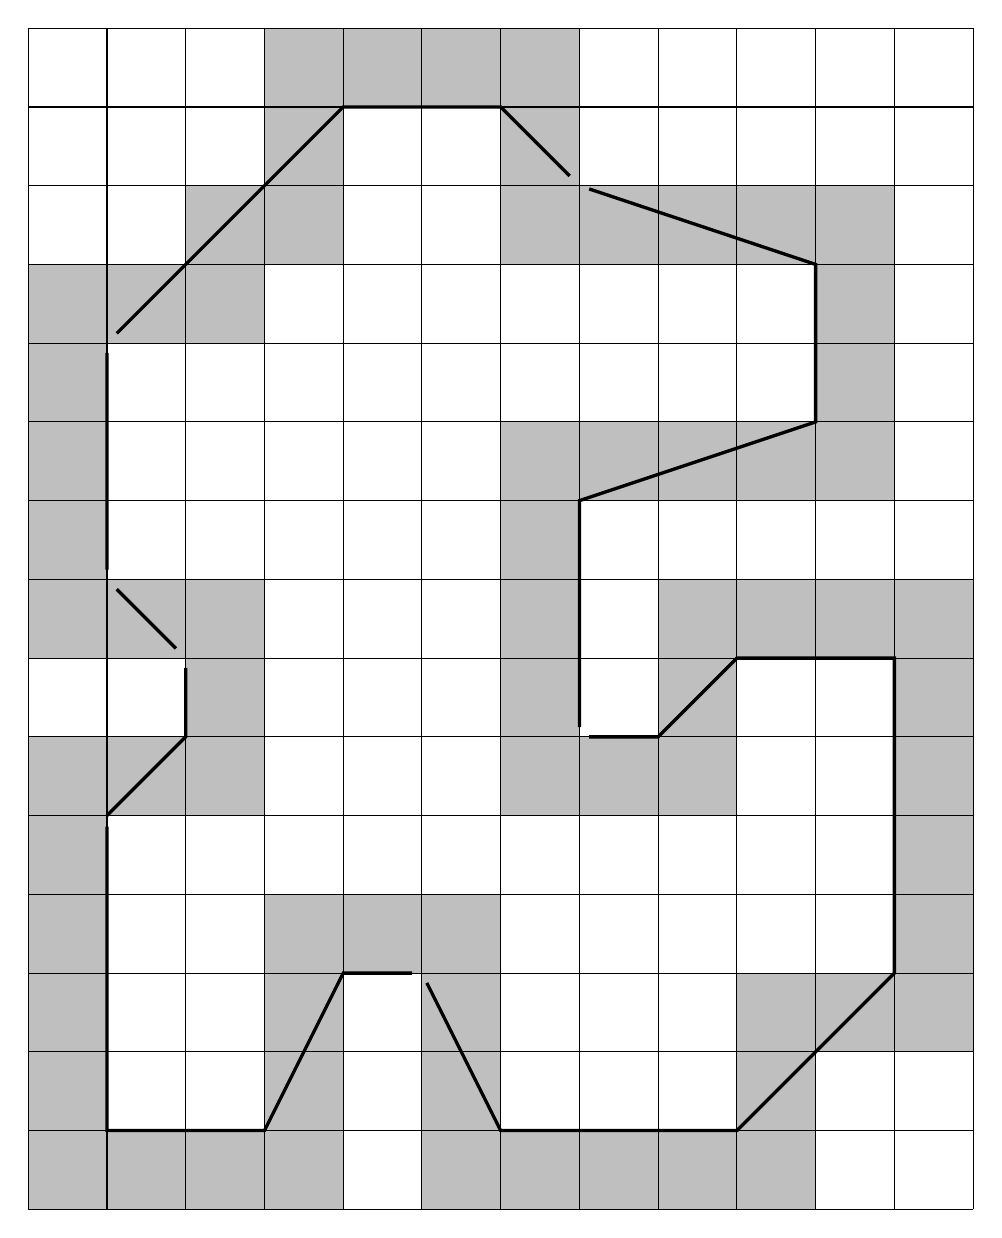
\begin{tikzpicture}

\draw [fill=lightgray] (0,12) rectangle (1,7)
 (1,8) node (v2) {} rectangle (3,7)
  (3,5) rectangle (2,7) node (v1) {}
  (2,5) rectangle (0,6)
  (0,5) rectangle (1,0)
  (1,0) rectangle (4,1)
  (4,1) rectangle (3,4)
  (4,4) rectangle (6,3)
  (5,3) node (v6) {} rectangle (6,0)
  (6,0) rectangle (10,1)
  (10,1) rectangle (9,3)
  (10,3) rectangle (12,2)
  (12,3) rectangle (11,8)
  (11,8) rectangle (8,7)
  (8,7) rectangle (9,5)
  (8,5) rectangle (6,6)
  (7,6) node (v5) {} rectangle (6,10)
  (7,10) rectangle (11,9)
 (11,10) rectangle (10,13)
  (10,13) rectangle (6,12)
  (7,13) node (v4) {} rectangle (6,15)
  (6,15) rectangle (3,14)
  (3,14) rectangle (4,12)
  (2,13) rectangle (3,11)
  (2,12) rectangle (1,11) node (v3) {};
  
 %\draw [very thick] plot[smooth, tension=.7] coordinates {(3.5,14.4) (6.5,14.3) (6.4,12.5) (9.9,12.5) (10.4,9.4) (6.8,9.5) (6.5,5.9) (8.6,5.5) (8.7,7.4) (11.4,7.3) (11.5,2.8) (9.4,2.4) (9.6,0.5) (7.1,0.4) (6.5,0.7) (5.7,0.4) (5.6,3.4) (4.6,3.3) (3.5,3.6) (3.4,0.6) (0.6,0.9) (0.7,5.5) (2.3,5.6) (2.5,7.7) (0.6,7.5) (0.4,11.4) (2.3,11.7) (2.5,12.3) (3.5,12.7) (3.4,13.3) (3.5,14.4)};

\foreach \x in {0,...,12} {
	\draw (\x,0) -- (\x,15);
}
\foreach \y in {0,...,15} {
	\draw (0,\y) -- (12,\y);
}

\draw [very thick] (1,5) node (v7) {} -- (2,6) -- (v1) -- (v2) -- (v3) -- (4,14) -- (6,14) -- (v4) -- (10,12) -- (10,10) -- (7,9) -- (v5) -- (8,6) -- (9,7) -- (11,7) -- (11,3) -- (9,1) -- (6,1) -- (v6) -- (4,3) -- (3,1) -- (1,1) -- (v7);
\end{tikzpicture}}
		\caption{Minimum perimeter polygon}
	\end{subfigure}
	\caption{MPP obtained by boundary shrinking}
\end{figure}

\begin{figure}[h]
	\centering
	\begin{subfigure}[b]{0.3\textwidth}
		\centering
		\adjustbox{scale=0.4}{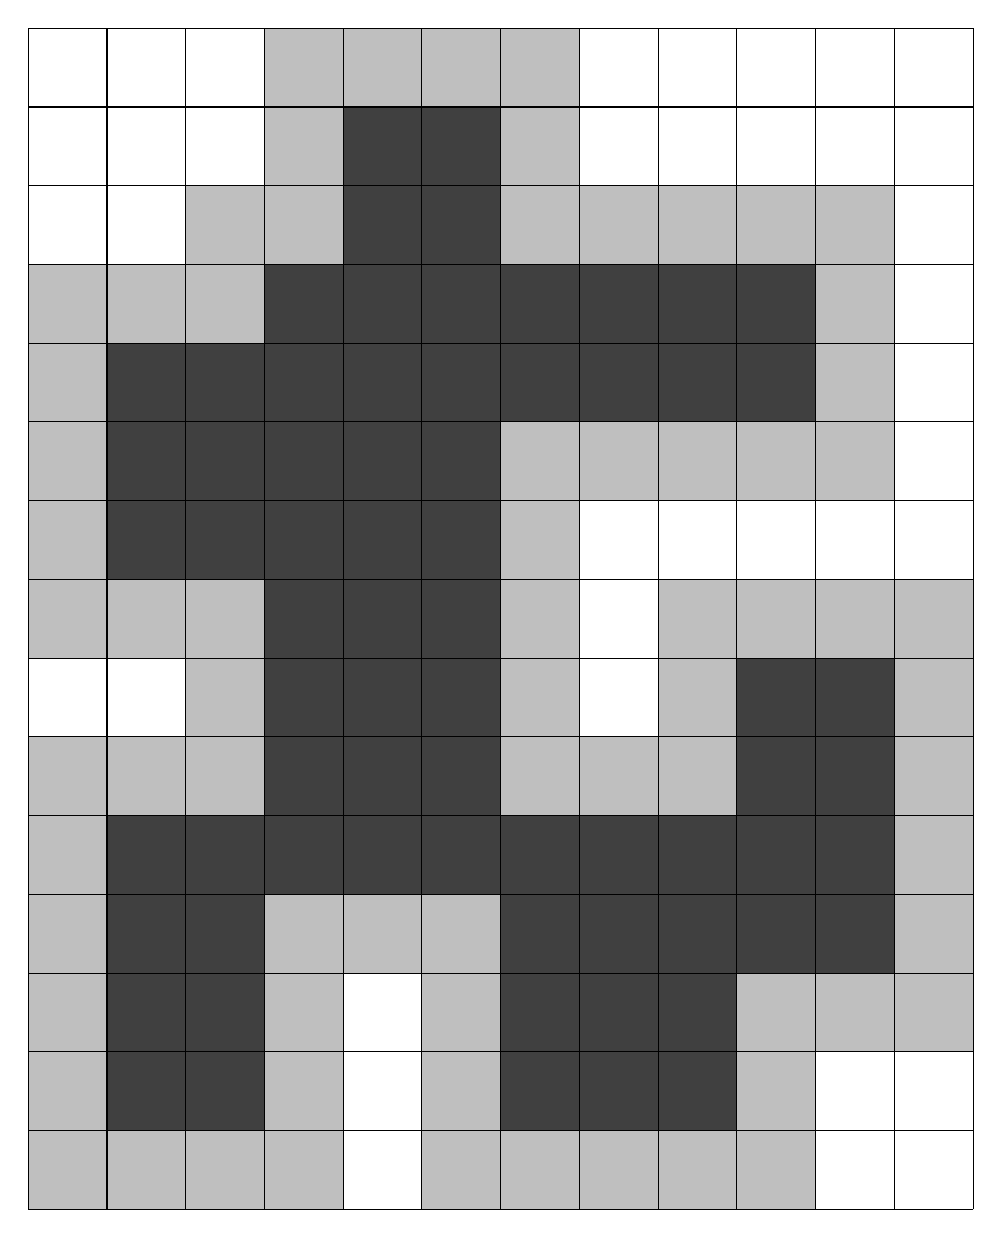
\begin{tikzpicture}

\draw [fill=lightgray] (0,12) rectangle (1,7)
 (1,8) node (v2) {} rectangle (3,7)
  (3,5) rectangle (2,7) node (v1) {}
  (2,5) rectangle (0,6)
  (0,5) rectangle (1,0)
  (1,0) rectangle (4,1)
  (4,1) rectangle (3,4)
  (4,4) rectangle (6,3)
  (5,3) node (v6) {} rectangle (6,0)
  (6,0) rectangle (10,1)
  (10,1) rectangle (9,3)
  (10,3) rectangle (12,2)
  (12,3) rectangle (11,8)
  (11,8) rectangle (8,7)
  (8,7) rectangle (9,5)
  (8,5) rectangle (6,6)
  (7,6) node (v5) {} rectangle (6,10)
  (7,10) rectangle (11,9)
 (11,10) rectangle (10,13)
  (10,13) rectangle (6,12)
  (7,13) node (v4) {} rectangle (6,15)
  (6,15) rectangle (3,14)
  (3,14) rectangle (4,12)
  (2,13) rectangle (3,11)
  (2,12) rectangle (1,11) node (v3) {};
  
\draw [fill=darkgray] (4,14) rectangle (6,12)
  (3,12) rectangle (10,10)
  (1,11) rectangle (3,8)
  (3,10) rectangle (6,4)
  (1,5) rectangle (3,1)
  (6,5) rectangle (9,1)
  (11,3) rectangle (9,7);
  
  
  
 %\draw [very thick] plot[smooth, tension=.7] coordinates {(3.5,14.4) (6.5,14.3) (6.4,12.5) (9.9,12.5) (10.4,9.4) (6.8,9.5) (6.5,5.9) (8.6,5.5) (8.7,7.4) (11.4,7.3) (11.5,2.8) (9.4,2.4) (9.6,0.5) (7.1,0.4) (6.5,0.7) (5.7,0.4) (5.6,3.4) (4.6,3.3) (3.5,3.6) (3.4,0.6) (0.6,0.9) (0.7,5.5) (2.3,5.6) (2.5,7.7) (0.6,7.5) (0.4,11.4) (2.3,11.7) (2.5,12.3) (3.5,12.7) (3.4,13.3) (3.5,14.4)};

\foreach \x in {0,...,12} {
	\draw (\x,0) -- (\x,15);
}
\foreach \y in {0,...,15} {
	\draw (0,\y) -- (12,\y);
}

%\draw [very thick] (1,5) node (v7) {} -- (2,6) -- (v1) -- (v2) -- (v3) -- (4,14) -- (6,14) -- (v4) -- (10,12) -- (10,10) -- (7,9) -- (v5) -- (8,6) -- (9,7) -- (11,7) -- (11,3) -- (9,1) -- (6,1) -- (v6) -- (4,3) -- (3,1) -- (1,1) -- (v7);

\end{tikzpicture}}
		\caption{Dark gray region resulting from enclosing the original boundary}
	\end{subfigure}
	\begin{subfigure}[b]{0.3\textwidth}
		\centering
		\adjustbox{scale=0.4}{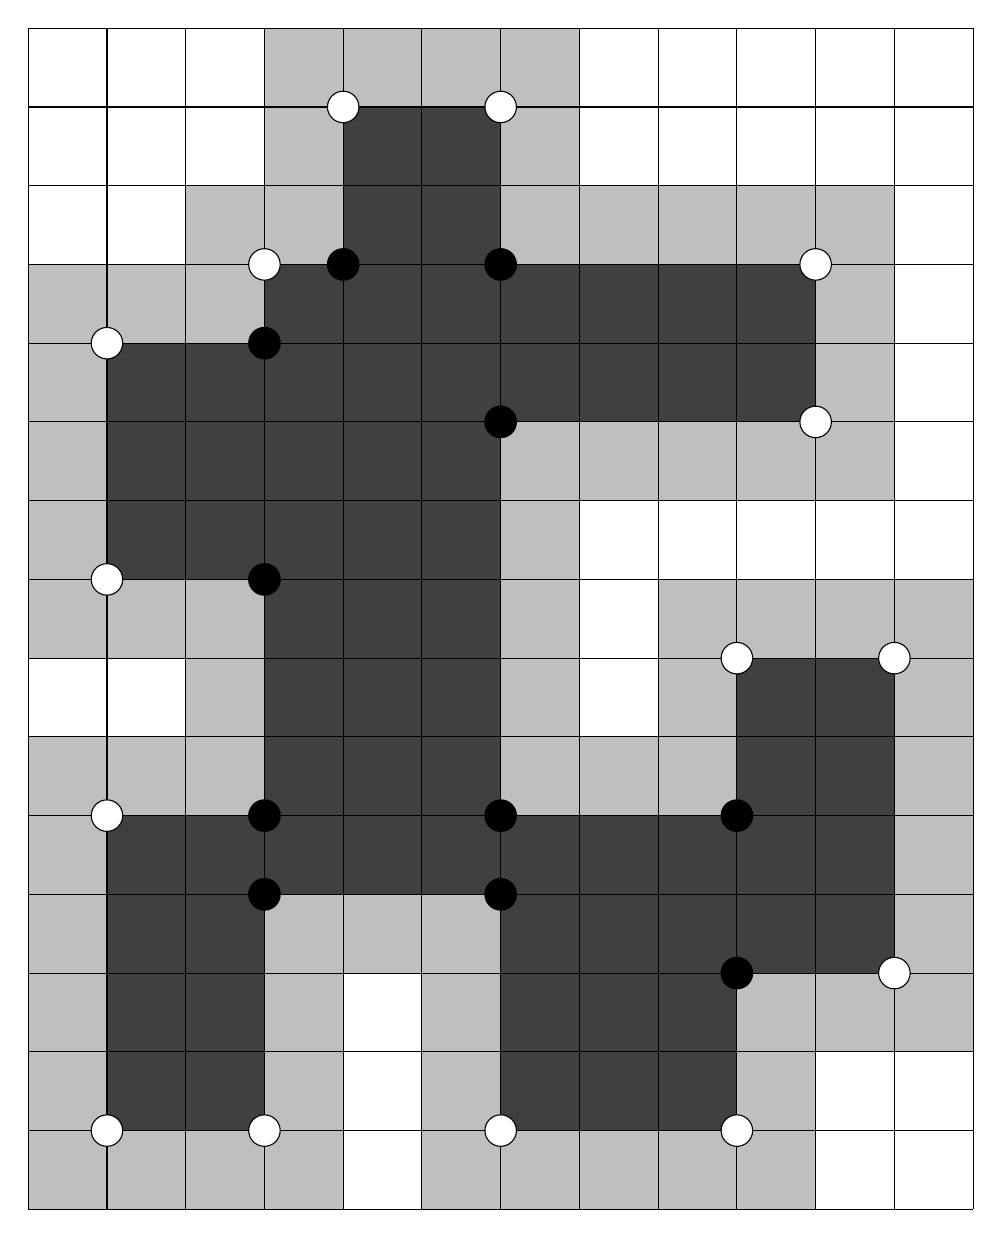
\begin{tikzpicture}

\draw [fill=lightgray] (0,12) rectangle (1,7)
 (1,8) node (v2) {} rectangle (3,7)
  (3,5) rectangle (2,7) node (v1) {}
  (2,5) rectangle (0,6)
  (0,5) rectangle (1,0)
  (1,0) rectangle (4,1)
  (4,1) rectangle (3,4)
  (4,4) rectangle (6,3)
  (5,3) node (v6) {} rectangle (6,0)
  (6,0) rectangle (10,1)
  (10,1) rectangle (9,3)
  (10,3) rectangle (12,2)
  (12,3) rectangle (11,8)
  (11,8) rectangle (8,7)
  (8,7) rectangle (9,5)
  (8,5) rectangle (6,6)
  (7,6) node (v5) {} rectangle (6,10)
  (7,10) rectangle (11,9)
 (11,10) rectangle (10,13)
  (10,13) rectangle (6,12)
  (7,13) node (v4) {} rectangle (6,15)
  (6,15) rectangle (3,14)
  (3,14) rectangle (4,12)
  (2,13) rectangle (3,11)
  (2,12) rectangle (1,11) node (v3) {};
  
\draw [fill=darkgray] (4,14) rectangle (6,12)
  (3,12) rectangle (10,10)
  (1,11) rectangle (3,8)
  (3,10) rectangle (6,4)
  (1,5) rectangle (3,1)
  (6,5) rectangle (9,1)
  (11,3) rectangle (9,7);
  
 %\draw [very thick] plot[smooth, tension=.7] coordinates {(3.5,14.4) (6.5,14.3) (6.4,12.5) (9.9,12.5) (10.4,9.4) (6.8,9.5) (6.5,5.9) (8.6,5.5) (8.7,7.4) (11.4,7.3) (11.5,2.8) (9.4,2.4) (9.6,0.5) (7.1,0.4) (6.5,0.7) (5.7,0.4) (5.6,3.4) (4.6,3.3) (3.5,3.6) (3.4,0.6) (0.6,0.9) (0.7,5.5) (2.3,5.6) (2.5,7.7) (0.6,7.5) (0.4,11.4) (2.3,11.7) (2.5,12.3) (3.5,12.7) (3.4,13.3) (3.5,14.4)};

\foreach \x in {0,...,12} {
	\draw (\x,0) -- (\x,15);
}
\foreach \y in {0,...,15} {
	\draw (0,\y) -- (12,\y);
}

%\draw [very thick] (1,5) node (v7) {} -- (2,6) -- (v1) -- (v2) -- (v3) -- (4,14) -- (6,14) -- (v4) -- (10,12) -- (10,10) -- (7,9) -- (v5) -- (8,6) -- (9,7) -- (11,7) -- (11,3) -- (9,1) -- (6,1) -- (v6) -- (4,3) -- (3,1) -- (1,1) -- (v7);

\foreach \x/\y in {1/1, 1/5, 1/8, 1/11, 3/12, 4/14, 6/14, 10/12, 10/10, 9/7, 11/7, 11/3, 9/1, 6/1, 3/1} {
	\draw [fill=white] (\x,\y) circle (0.2);
}
\foreach \x/\y in {3/5, 3/8, 3/11, 4/12, 6/12, 6/10, 6/5, 9/5, 9/3, 6/4, 3/4} {
	\draw [fill=black] (\x,\y) circle (0.2);
}

\end{tikzpicture}}
		\caption{Convex (white) and concave (black) vertices}
	\end{subfigure}
	\begin{subfigure}[b]{0.3\textwidth}
		\centering
		\adjustbox{scale=0.4}{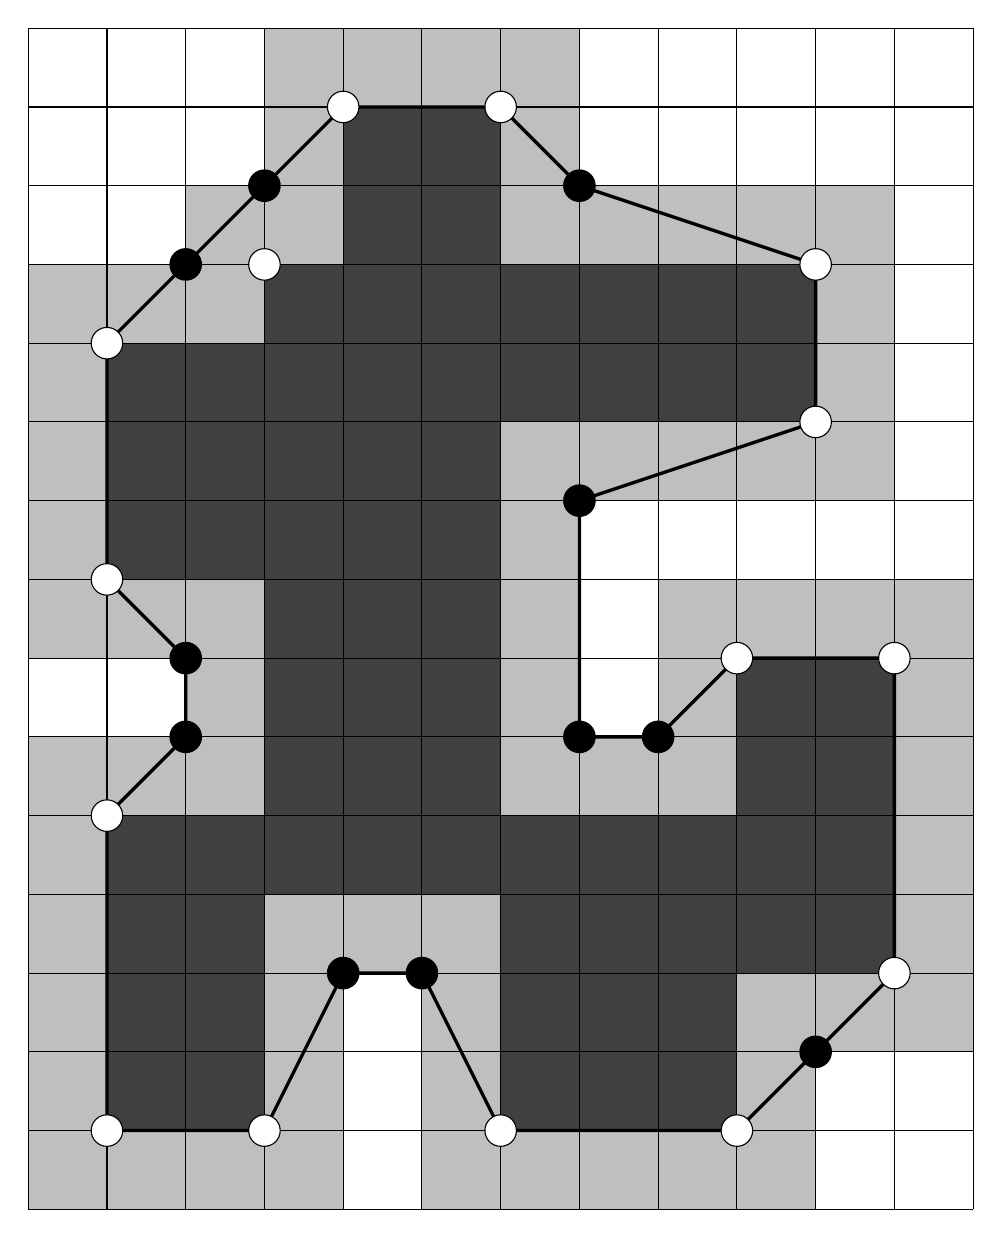
\begin{tikzpicture}

\draw [fill=lightgray] (0,12) rectangle (1,7)
 (1,8) node (v2) {} rectangle (3,7)
  (3,5) rectangle (2,7) node (v1) {}
  (2,5) rectangle (0,6)
  (0,5) rectangle (1,0)
  (1,0) rectangle (4,1)
  (4,1) rectangle (3,4)
  (4,4) rectangle (6,3)
  (5,3) node (v6) {} rectangle (6,0)
  (6,0) rectangle (10,1)
  (10,1) rectangle (9,3)
  (10,3) rectangle (12,2)
  (12,3) rectangle (11,8)
  (11,8) rectangle (8,7)
  (8,7) rectangle (9,5)
  (8,5) rectangle (6,6)
  (7,6) node (v5) {} rectangle (6,10)
  (7,10) rectangle (11,9)
 (11,10) rectangle (10,13)
  (10,13) rectangle (6,12)
  (7,13) node (v4) {} rectangle (6,15)
  (6,15) rectangle (3,14)
  (3,14) rectangle (4,12)
  (2,13) rectangle (3,11)
  (2,12) rectangle (1,11) node (v3) {};
  
\draw [fill=darkgray] (4,14) rectangle (6,12)
  (3,12) rectangle (10,10)
  (1,11) rectangle (3,8)
  (3,10) rectangle (6,4)
  (1,5) rectangle (3,1)
  (6,5) rectangle (9,1)
  (11,3) rectangle (9,7);
  
 %\draw [very thick] plot[smooth, tension=.7] coordinates {(3.5,14.4) (6.5,14.3) (6.4,12.5) (9.9,12.5) (10.4,9.4) (6.8,9.5) (6.5,5.9) (8.6,5.5) (8.7,7.4) (11.4,7.3) (11.5,2.8) (9.4,2.4) (9.6,0.5) (7.1,0.4) (6.5,0.7) (5.7,0.4) (5.6,3.4) (4.6,3.3) (3.5,3.6) (3.4,0.6) (0.6,0.9) (0.7,5.5) (2.3,5.6) (2.5,7.7) (0.6,7.5) (0.4,11.4) (2.3,11.7) (2.5,12.3) (3.5,12.7) (3.4,13.3) (3.5,14.4)};

\foreach \x in {0,...,12} {
	\draw (\x,0) -- (\x,15);
}
\foreach \y in {0,...,15} {
	\draw (0,\y) -- (12,\y);
}

\draw [very thick] (1,5) node (v7) {} -- (2,6) -- (v1) -- (v2) -- (v3) -- (4,14) -- (6,14) -- (v4) -- (10,12) -- (10,10) -- (7,9) -- (v5) -- (8,6) -- (9,7) -- (11,7) -- (11,3) -- (9,1) -- (6,1) -- (v6) -- (4,3) -- (3,1) -- (1,1) -- (v7);

\foreach \x/\y in {1/1, 1/5, 1/8, 1/11, 3/12, 4/14, 6/14, 10/12, 10/10, 9/7, 11/7, 11/3, 9/1, 6/1, 3/1} {
	\draw [fill=white] (\x,\y) circle (0.2);
}
\foreach \x/\y in {2/6, 2/7, 2/12, 3/13, 7/13, 7/9, 7/6, 8/6, 10/2, 5/3, 4/3} {
	\draw [fill=black] (\x,\y) circle (0.2);
}

\end{tikzpicture}}
		\caption{Concave vertices displaced to their diagonal mirror locations}
	\end{subfigure}
	\caption{MPP obtained by boundary shrinking}
\end{figure}

\begin{enumerate}
\item Find all convex points (white dots) and concave points (black dots).
\item Mirror the concave points to their diagonal location in the outer wall.
\item The orientation (cw or ccw) of a sequence of three points will be necessary. This replaces the convec concave classification
\begin{enumerate}
\item $a=(x_1, y_1), b=(x_2, y_2), c=(x_3, y_3)$
\item $A=\begin{bmatrix}
	x_1 & y_1 & 1\\
  	x_2 & y_2 & 1\\
  	x_3 & y_3 & 1\\
\end{bmatrix}$
\item $det(A) =$ 
\begin{itemize}
\item $> 0$ if $(a, b, c)$ is a counterclockwise sequence
\item $= 0$ if the points are collinear
\item $< 0$ if $(a, b, c)$ is a clockwise sequence
\end{itemize}
\end{enumerate}
\item For notational convenience let $sgn(a,b,c) = det(A)$
\item Names
\begin{itemize}
\item $V_L$ are found vertices of the MPP
\item $V_K$ is the next possible candidate
\item $B_C$ is a black vertex
\item $W_C$ is a white vertex
\end{itemize} 
\item $V_K$ lies to the positive side of the line through pair ($V_L$, $W_C$), that is $sgn(V_L, W_C, V_K)>0$. If this condition holds, the next MPP vertex is $W_C$
\item $V_K$ lies to the negative side of the line through pair ($V_L$, $B_C$), that is $sgn(V_L, B_C, V_K)<0$. If this condition holds, the next MPP vertex is $B_C$.
\item $V_K$ lies on the negative side of the line through pair ($V_L$, $W_C$) or is collinear with it, that is $sgn(V_L, W_C, V_K) \le 0$. At the same time, $V_K$ lies on the positive side of the line through ($V_L$, $B_C$) or is collinear with it, that is $sgn(V_L, V_C, V_K) \ge 0$. If this condition holds, the next candidate MPP vertex is $V_K$; otherwise $B_C = V_K$
\item Continue with the next vertex in the list.
\end{enumerate}

\subsubsection{Other Polygonal Approximation Approaches\buchSeite{807}}
\paragraph{Merging\buchSeite{807}}
Points on the boundary are merged and a line is fitted to these points. 
If the fitting error becomes to large, a vertex is set and the procedure starts from the beginning.
This approach is very simple, but there is no guarantee for a good approximation.
E.g. it does not set vertices at corners, but always a bit later. 

\paragraph{Splitting\buchSeite{808}}
Here the idea is, to divide (split) a boundary segment until a threshold of an criterion is satisfied.
E.g. until the distances from the boundary to the approximated lines are below a certain number.

\subsubsection{Signatures\buchSeite{808}}
A signature is a 1D function that represents a boundary. This results in a significant complexity reduction. There are several schemes:\\
\begin{itemize}
\item Find the centroid. The boundary is described as a function of the angle around this point.
\begin{itemize}
\item Rotational invariance: this can be achieved by selecting the point on the eigen axis that is farthest from the centroid.
\item Scaling invariance: this can be achieved by dividing the signature by its standard deviation.
\end{itemize}
\end{itemize}
\begin{figure}[h]
	\begin{subfigure}{0.5\textwidth}
		\centering
		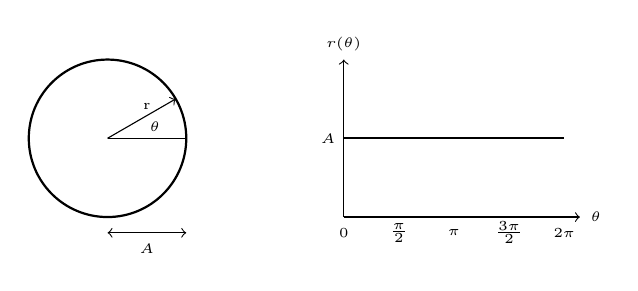
\begin{tikzpicture}

% Circle
\node[draw,thick,circle,minimum size=2cm] at (0,0) {};
\draw (0,0) -- (1,0);
\draw[->] (0,0) -- (0.866,0.5);
\node at (0.5,0.4) {\tiny r};
\node at (0.6,0.15) {\tiny $\theta$};
\draw[<->] (0,-1.2) -- (1,-1.2);
\node at (0.5,-1.4) {\tiny $A$};

% Signature

\draw[->] (3,-1) -- (6,-1);
\draw[->] (3,-1) -- (3,1);
\node at (3,1.2) {\tiny $r(\theta)$};
\node at (6.2,-1) {\tiny $\theta$};

\node at (3,-1.2) {\tiny $0$};
\node at (3.7,-1.2) {\tiny $\frac{\pi}{2}$};
\node at (4.4,-1.2) {\tiny $\pi$};
\node at (5.1,-1.2) {\tiny $\frac{3\pi}{2}$};
\node at (5.8,-1.2) {\tiny $2\pi$};

\node at (2.8,0) {\tiny $A$};

\draw[thick] (3,0) -- (5.8,0);

\end{tikzpicture}
		\caption{Signature of a circle}
	\end{subfigure}
	\begin{subfigure}{0.5\textwidth}
		\centering
		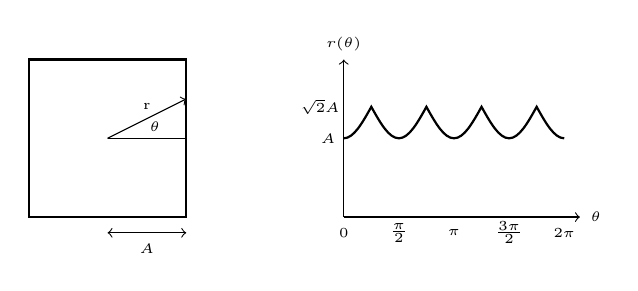
\begin{tikzpicture}

% Circle
\node[draw,thick,rectangle,minimum size=2cm] at (0,0) {};
\draw (0,0) -- (1,0);
\draw[->] (0,0) -- (1,0.5);
\node at (0.5,0.4) {\tiny r};
\node at (0.6,0.15) {\tiny $\theta$};
\draw[<->] (0,-1.2) -- (1,-1.2);
\node at (0.5,-1.4) {\tiny $A$};

% Signature

\draw[->] (3,-1) -- (6,-1);
\draw[->] (3,-1) -- (3,1);
\node at (3,1.2) {\tiny $r(\theta)$};
\node at (6.2,-1) {\tiny $\theta$};

\node at (3,-1.2) {\tiny $0$};
\node at (3.7,-1.2) {\tiny $\frac{\pi}{2}$};
\node at (4.4,-1.2) {\tiny $\pi$};
\node at (5.1,-1.2) {\tiny $\frac{3\pi}{2}$};
\node at (5.8,-1.2) {\tiny $2\pi$};

\node at (2.7,0.4) {\tiny $\sqrt{2}A$};
\node at (2.8,0) {\tiny $A$};

\draw[thick] (5.8,0) cos (5.45,0.4) sin (5.1,0) cos (4.75,0.4) sin (4.4,0) cos (4.05,0.4) sin (3.7,0) cos (3.35,0.4) sin (3,0);

\end{tikzpicture}
		\caption{Signature of a square}
	\end{subfigure}
	\caption{Examples for signatures}
\end{figure}

\subsubsection{Boundary segments\buchSeite{810}}
The convex hull H of an arbitrary set S is the smallest convex set containing S. The difference $D=H-S$ is the convex deficiency. Follow the contour of S and mark the spots where the contour makes a transition into or out of D. These marking $\alpha$ (0...1) are relative to the total length of the contour D.\\
This is in theory invariant to:\\
\begin{itemize}
\item Rotation
\item Translation
\item Scaling
\end{itemize}
In practice, boundaries have some noise. Often smooting along the boundaries is used.\\
\subsubsection{Skeletons\buchSeite{812}}
Medial axis transform (MAT)
\begin{itemize}
\item Every point in the region finds its closest boundary point.
\item If a point in the region has two closest boundary points, it belongs to the skeleton of the region.
\item Direct implementation of this is computationally expensive.
\end{itemize}
Algorithms for efficient MAT iteratively delete boundary points subject to
\begin{enumerate}
\item keep end points
\item keep connectivity (\small note that morphological thinning does \emph{not} account for this)
\item do not erode that region excessively
\end{enumerate}
Thinning algorithm is 2 steps applied successively to border points\\
\begin{tikzpicture}
\matrix[3x3mask]{
p9 & p2 & p3 \\
p8 & p1 & p4 \\
p7 & p6 & p5 \\
};\\
\end{tikzpicture}\\
\paragraph{Step 1:} south or east boundary points\\
Flag for deletion if all of these conditions are satisfied:
\begin{enumerate}[label={\alph*)}]
\item $2\leq N(P_1)\leq 6$ with $N(p_1)=p_2 + p_3 + \ldots + p_9$
\item $T(p_1)=1$ where $T(p_1)$ is the number of $0-1$ transitions in the ordered sequence $p_2,p_3,\ldots ,p_8,p_9,p_2$
\item $p_2 \cdot p_4 \cdot p_6 = 0$
\item $p_4 \cdot p_6 \cdot p_8 = 0$
\end{enumerate}
The last conditions are satisfied simultaneously by the minimum set of values: $(p_4=0\ or\ p_6=0)\ or \ (p_2=0\ \text{and} \ p_8=0)$\\
After processing all boundary points, the marked ones are deleted\\
\paragraph{Step 2:} north or west boundary points\\
Simultaneous to Step 1 except the new conditions $c'$ and $d'$\\
\begin{enumerate}[label={\alph*)}]
\item $2\leq N(P_1)\leq 6$ with $N(p_1)=p_2 + p_3 + \ldots + p_9$
\item $T(p_1)=1$ where $T(p_1)$ is the number of $0-1$ transitions in the ordered sequence $p_2,p_3,\ldots ,p_8,p_9,p_2$
\end{enumerate}
\begin{enumerate}[label={\alph*')},resume]
\item $p_2 \cdot p_4 \cdot p_8 = 0$
\item $p_2 \cdot p_6 \cdot p_8 = 0$
\end{enumerate}

\subsection{Boundary Descriptors\buchSeite{815}}
\label{sec:boundaryDescriptors}
Having seen different representations of boundaries, the goal is now to develop descriptors for these boundaries.
\subsubsection{Simple Descriptors\buchSeite{815}}

\paragraph{Length}
\begin{itemize}
\item Number of pixels along a Boundary gives a rough approximation of its length
\item 8-directional Chain Code numbers of vertical and horizontal components plus $\sqrt{2}$ times the number of diagonal components, gives the exact length.
\end{itemize}
\paragraph{Diameter of boundary B}

\begin{flalign*}
& \text{Diam}(B)=\max\limits_{i,j}\left[D(p_i,p_j)\right] && \text{Points on boundary:} && p_i,p_j && \text{Distance measure:} && D 
\end{flalign*}

\paragraph{Major axis}
The line connecting the two extreme points of the boundary is called the major axis of the boundary.\\
\paragraph{Minor axis}
The line perpendicular to the major axis and of such length that a box passing through the outer four points of intersection ofthe boundary with the two axes completely encloses the boundary.
\paragraph{Eccentricity}
The ratio of the major to the minor axis is called the eccentricity of the boundary. This is a useful descriptor.
\paragraph{Curvature}
This is the rate of change of the slope in the boundary. i.e. this is a second derivative. 
Note that the curvature is often very noisy. It is therefore often applied to a polygon approximation.

\subsubsection{Shape numbers\buchSeite{816}}
The shape number of a boundary (based on 4-directional code) is defined as the first difference of smalles magnitude.\\
The order n of a shape number is defined as the number of digits in its representation.\\
One way of aligning the chain code grid with the boundary is to use the basic rectangle box based on the major and minor axes\\

\subsubsection{Fourier descriptors\buchSeite{818}}
The coordinates of the boundary represents a complex sampled signal wich can be represented as a complex vector 
\begin{align*}
s(k)=x(k)+jy(k) && k=0,1,2,\ldots,K-1
\end{align*} 
which can be analyzed in the frequency domain.\\

Note that the axis are changed:
\begin{figure}[h]
	\begin{subfigure}{0.5\textwidth}
		 \centering
		 \begin{tikzpicture}[scale=0.5]

\draw[thick,->](0,0) -- (4,0);
\draw[thick,->](0,0) -- (0,-2);

\node at (4.3,0) {y};
\node at (0,-2.3) {x};

\end{tikzpicture}
		 \caption{Normal}
	\end{subfigure}
	\begin{subfigure}{0.5\textwidth}
		\centering
		\begin{tikzpicture}[scale=0.5]

\draw[thick,->](0,0) -- (4,0);
\draw[thick,->](0,0) -- (0,2);

\node at (4.3,0) {x};
\node at (0,2.3) {jy};

\end{tikzpicture}
		\caption{for Fourier descriptors}
	\end{subfigure}
	\caption{Axes of image}
\end{figure}

The DFT of $s(k)$ is \begin{align*}
& \text{Fourier descriptors of the boundary:} && a(u)=\sum\limits_{k=0}^{K-1}s(k)e^{-j2\pi uk/K} && u=0,1,2,\ldots,K-1\\
& \text{Inverse Fourier transform:} && s(k)=\frac{1}{K}\sum\limits_{u=0}^{K-1}a(u)e^{j2\pi uk/K}
\end{align*} 

Since the high frequency components are responsible for the fine detail, using only the first few Fourier descriptors results in a smoothing of the boundary and image compression.\\
The reconstruction of the image is, when using the first $P$ coefficients
	\[
	\hat{s}(k) = \frac{1}{K} \sum\limits_{u=0}^{P-1} a(u) e^{j 2 \pi u k / K}
	\]

\paragraph{Basic properties of Fourier descriptors} ~\\

\begin{tabularx}{\textwidth}{XXX}
Transformation & Boundary & Fourier Descriptor \\\hline
Identity & $s(k)$ & $a(u)$ \\
Rotation & $s_r(k)=s(k)e^{j\theta}$& $a_r(u)=a(u)e^{j\theta}$ \\
Translation &$s_t(k)=s(k)+\Delta_{xy}$& $a_t(u)=a(u)+\Delta_{xy}\delta(u)$ \\
Scaling &$s_s(k)=\alpha s(k)$& $a_s(u)=\alpha a(u)$ \\
Starting point & $s_p(k)=s(k-k_0)$& $a_p(u)=a(u)e^{-j2\pi k_0u/K}$ \\ \hline
\end{tabularx}

\subsubsection{Statistical moments\buchSeite{821}}
The boundary segment is rotated, so that it can be interpreted as a function of a single variable. \\

The amplitude of $g()$ can be treated as a discrete random variable v and a amplitude histogram $p(v_i)$ can be formed. 
From the histogram, the statistical moments can be calculated.

\begin{align*}
	m &= \sum\limits_{i=0}^{A-1} v_i p(v_i) \\
	\mu_n(v) &= \sum\limits_{i=0}^{A-1} (v_i-m)^n p(v_i)
\end{align*}

The statistical moments are:
\begin{itemize}
\item $m$ or $\mu_1$: Mean
\item $\mu_2$: Variance
\item $\mu_3$: Skewness (this is a measure of asymmetry)
\item $\mu_4$: Kurtosis (peakedness)
\end{itemize}

If $g()$ is normalized such that it represents a probability density function (pdf), i.e. it sums up to 1, 
the histogram building can be skipped and $g()$ can directly be analyzed by statistical moments.

\subsection{Regional descriptors\buchSeite{822}}
\subsubsection{Simple descriptors\buchSeite{822}}
\begin{itemize}
\item Area: Number of pixels
\item Perimeter: Lenght of boundary
\item Compactness: $\text{Perimeter}^2/\text{area}$
\item Circularity ratio $R_C=\frac{4\pi A}{P^2}$ where $A$ is the area of the region in question and $P$ the length of its perimeter
\item Mean, median, minimum, maximum of intensity
\item Etc.
\end{itemize}
\subsubsection{Topological descriptors\buchSeite{823}}
Topological descriptors are descriptors that do not change under rubber-sheet distortions. No tearing, no folding allowed.\\
The number of holes $H$ and connected components $C$ in a figure can be used to define the Euler number $E=C-H$\\

\begin{figure}[h]
	\centering
	\adjustbox{scale=1.2}{\begin{tikzpicture}

\draw [fill=lightgray] (0,0) -- (1,0.5) -- (0.5,1) -- cycle;
\draw [fill=lightgray] (2.5,1) -- (1,0.5) -- (3.5,0.5) -- cycle;

\draw (0,0) node [circ] {} -- (0.5,1) node [circ] {} -- (1.5,1.5) node [circ] {} -- (2.5,1) node [circ] {} -- (3.5,0.5) node [circ] {} -- (2,-0.5) node [circ] {} -- (0,0);
\draw (1,0.5) node [circ] {} -- (0.5,1);
\draw (1,0.5) -- (2.5,1);
\draw (1,0.5) -- (3.5,0.5);
\draw (1,0.5) -- (2,-0.5);
\draw (1,0.5) -- (0,0);

%labels

\draw[->] (2,2)  node [anchor=west] {Vertex} -- (1.5,2) -- (1.5,1.7);
\draw[->] (3.5,1.5)  node [anchor=west] {Face} -- (3,1.5) -- (2.5,0.7);
\draw[->] (3,-0.5)  node [anchor=west] {Hole} -- (2.5,-0.5) -- (2,0);
\draw[->] (1.5,-1)  node [anchor=west] {Edge} -- (1,-1) -- (1,-0.25);



\draw  plot[smooth, tension=.7] coordinates {(-1,0) (-0.2,1.6) (0.5,2.6) (2.7,2.6) (4.5,2.5) (5.8,1.3) (4.8,0.5) (4.2,-0.9) (2.8,-1.6) (0.5,-1.6) (-0.8,-0.9) (-1,0)};
\end{tikzpicture}}
	\caption{A region containing a polygonal network}
	
	In this example: \\
	\begin{align*}
	V=7 \quad Q=11 \quad F=2 \qquad &\Rightarrow E=-2 \\
	C=1 \quad H=3 \qquad &\Rightarrow E=-2
	\end{align*}

\end{figure}

\begin{itemize}
\item Number of vertices V
\item Number of edges Q
\item Number of faces F
\end{itemize}
Euler proved that $E=V-Q+F=C-H$
\subsubsection{Texture\buchSeite{827}}
Smoothness, coarseness, regularity etc.\\
There are three basic approaches to describe texture:\\

\paragraph{Statistical approaches\buchSeite{828}}
\begin{itemize}
\item Intensity histogram $p(z_i)$
\item Moment $\mu_n(z)=\sum\limits_{i=0}^{L-1}(z_i-m)^np(z_i)$ and mean $m=\sum\limits_{i=0}^{L-1}z_ip(z_i)$
\item The variance $\sigma ^2(z) =\mu_2 (z)$ is a measure of contrast, which can be used to establish descriptors of smoothness. It should be normalized to $0 \ldots 1$ by dividing by $\left(\frac{L-1}{2}\right)^2$. $R(z)=1-\frac{1}{1+\sigma ^2(z)}$
\item A measure for uniformity $U(z)=\sum\limits_{i=0}^{L-1}p^2(z_i)$
\item Average entropy $e(z)=-\sum\limits_{i=0}^{L-1}p(z_i)\log_2p(z_i)$ \\ Note that $e$ is zero for constant regions.
\end{itemize}

\paragraph{Relative positions} Measures with only histograms have no information about the relative positions of pixels with respect to each other.
Thus, a $Q$ operator, that defines the positions of two pixels relative to each other, is introduced. 
A \emph{co-occurrence matrix} $\mathbf{G}$ is generated, whose elements $g_{i,j}$ are how many times a certain pixel pair $(z_i,z_j)$ appears. \\

\begin{figure}[h]
	\centering
	\begin{tikzpicture}

	% Image
	\matrix(dict)[matrix of nodes, nodes={inner sep=0pt,text width=0.5cm, minimum height=0.5cm, align=center}] at (0,0) {
		1 & 1 & 7 & 5 & 3 & 2 \\
		5 & 1 & 6 & 1 & 2 & 5 \\
		8 & 8 & 6 & 8 & 1 & 2 \\
		4 & 3 & 4 & 5 & 5 & 1 \\
		8 & 7 & 8 & 7 & 6 & 2 \\
		7 & 8 & 6 & 2 & 6 & 2 \\
	};
	\draw[help lines,step=0.5] (-1.5,-1.5) grid (1.5,1.5);
	
	% Co-occurrence matrix
	\matrix(dict)[matrix of nodes, nodes={inner sep=0pt,text width=0.5cm, minimum height=0.5cm, align=center}] at (6.75,0.25) {
	  & 1 & 2 & 3 & 4 & 5 & 6 & 7 & 8  \\
	1 & 1 & 2 & 0 & 0 & 0 & 1 & 1 & 0 \\
	2 & 0 & 0 & 0 & 0 & 1 & 1 & 0 & 0 \\
	3 & 0 & 1 & 0 & 1 & 0 & 0 & 0 & 0 \\
	4 & 0 & 0 & 1 & 0 & 1 & 0 & 0 & 0 \\
	5 & 2 & 0 & 1 & 0 & 1 & 0 & 0 & 0 \\
	6 & 1 & 3 & 0 & 0 & 0 & 0 & 0 & 1 \\
	7 & 0 & 0 & 0 & 0 & 1 & 1 & 0 & 2 \\
	8 & 1 & 0 & 0 & 0 & 0 & 2 & 2 & 1 \\
	};
	\draw[help lines,step=0.5] (5.0,-2) grid (9,2);
	\draw[help lines] (5.0,-2) -- (5.0,2);
	
	% generation
	\draw (-1.0,1.25) ellipse (0.48cm and 0.24cm);
	\draw[->] (-1,1.49) .. controls (-0.5,2) and (1.5,2.5) .. (5.1,1.8);

\end{tikzpicture}
	\caption{Co-occurrence matrix $\mathbf{G}$}
\end{figure}

\begin{table}[h]
	\begin{tabular}{lll}
		$n$	& & sum of elements in $\mathbf{G}$ \\
		$K$ & & size of co-occurrence matrix $\mathbf{G}$ (size: $K \times K$) \\
		$g_{ij}$ & & element of $\mathbf{G}$ \\
		$p_{ij}$ & $= g_{i,j} / n$ & estimate for probability of a pair $(z_i,z_j)$ \\
		$m_r$ &= $\sum\limits_{i=1}^{K} i \sum\limits_{j=1}^{K} p_{ij}$ & mean, computed along rows of $\mathbf{G}$ \\
		$m_c$ &= $\sum\limits_{j=1}^{K} j \sum\limits_{i=1}^{K} p_{ij}$ & mean, computed along columns of $\mathbf{G}$ \\
		$\sigma_r^2$ &= $\sum\limits_{i=1}^{K} (i-m_r)^2 \sum\limits_{j=1}^{K} p_{ij}$ & variance, computed along rows of $\mathbf{G}$ \\
		$\sigma_c^2$ &= $\sum\limits_{j=1}^{K} (j-m_r)^2 \sum\limits_{i=1}^{K} p_{ij}$ & variance, computed along columns of $\mathbf{G}$ \\
	\end{tabular}
\end{table}

First, all probabilities $p_{ij}$ and the means $m_r, m_c$ and variances $\sigma_r^2,\sigma_c^2$ are calculated. 
Then, the following descriptors can be calculated, if needed. Note that the correlation and the entropy are the most common descriptors.

\begin{table}[h]
	\begin{tabularx}{\textwidth}{lXl}
		\textbf{Descriptor} & \textbf{Explanation} & \textbf{Formula} \\ \hline
		Maximum probability & Measures the strongest response of $\mathbf{G}$. The range of values is $[0,1]$. & $\displaystyle\max_{i,j}(p_{ij})$ \\
		Correlation & A measure of how correlated a pixel is to its neighbor over the entire image. Range of values is $1$ to $-1$, corresponding to perfect positive or negative correlations. & $\displaystyle\sum\limits_{i=1}^{K}\sum\limits_{j=1}^{K}\frac{(i-m_r)(j-m_c)p_{ij}}{\sigma_r \sigma_c}$ \\
		Contrast & A measure of intensity contrast between a pixel and its neighbor over the entire image. The range of values is $0$ (when $\mathbf{G}$ is constant) to $(K-1)^2$. & $\displaystyle\sum\limits_{i=1}^{K}\sum\limits_{j=1}^{K}(i-j)^2 p_{ij}$ \\
		Uniformity (Energy) & A measure of uniformity in the range $[0,1]$. Uniformity is $1$ for a constant image. & $\displaystyle\sum\limits_{i=1}^{K}\sum\limits_{j=1}^{K} p_{ij}^2$ \\
		Homogeneity & Measures the spatial closeness of the distribution of elements in $\mathbf{G}$ to the diagonal. The range of values is $[0,1]$, with the maximum being achieved when $\mathbf{G}$ is a diagonal matrix. & $\displaystyle\sum\limits_{i=1}^{K}\sum\limits_{j=1}^{K}\frac{p_{ij}}{1+|i-j|}$ \\
		Entropy & Measures the randomness of the elements of $\mathbf{G}$. The entropy is $0$ when all $p_{ij}$'s are $0$ and is maximum when all $p_{ij}$'s are equal. The maximum value is $2 \log_2 K$. & $\displaystyle -\sum\limits_{i=1}^{K}\sum\limits_{j=1}^{K} p_{ij} \log_2 p_{ij}$ \\
		\hline
	\end{tabularx}
\end{table}


\paragraph{Structural approaches\buchSeite{836}}
Some texture can be described as a repetition of a simple primitive. For such textures, a description based on rewriting rules is useful.

\paragraph{Spectral approaches\buchSeite{837}}
Good for periodic patterns\\
The energy spectrum $S(r,\theta)$ is analyzed in polar coordinates. It is analyzed for a fixed angle, $S_\theta(r)$ and/or a fixed radius $S_r(\theta)$. The advantage of this is, that these are 1D functions and therefore easier to deal with.\\
$S(r)=\sum\limits_{\theta = 0}^{\pi}S_\theta(r)$\\
$S(\theta)=\sum\limits_{r=1}^{R_0}S_r(\theta)$\\
\subsubsection{Moment Invariants\buchSeite{839}}
A set of seven moments for a given image region can be generated as regional descriptors. They are intrinsically invariant to translation, scale change, rotation and even mirroring except for a sign change.\\
\begin{tabular}{ll}
2D moments of order (p+q) & $m_{pq}=\sum\limits_{x=0}^{M-1}\sum\limits_{y=0}^{N-1}x^py^qf(x,y)$ \\
The central moments & $\mu_{pq}=\sum\limits_{x=0}^{M-1}\sum\limits_{y=0}^{N-1}(x-\overline{x})^p(y-\overline{y})^qf(x,y)$ \\
& $\overline{x}=\frac{m_{10}}{m_{00}}$ and $\overline{y}=\frac{m_{01}}{m_{00}}$ \\
Normalized central moments & $ \eta_{pq}=\frac{\mu_{pq}}{\mu_{00}^\gamma} $ with $\gamma=\frac{p+q}{2}+1 $ \\
\end{tabular}
The seven invariant moments:\\
\begin{align*}
\phi_1 =& \eta_{20}+\eta_{02} \\
\phi_2 =& (\eta_{20}-\eta_{02})^2+4\eta_{11}^2 \\
\phi_3 =& (\eta_{30}-3\eta_{12})^2+(3\eta_{21}-\eta_{03})^2 \\
\phi_4 =& (\eta_{30}+\eta_{12})^2+(\eta_{21}+\eta_{03})^2 \\
\phi_5 =& (\eta_{30}-3\eta_{12})(\eta_{30}+\eta_{12})[(\eta_{30}+\eta_{12})^2-3(\eta_{21}+\eta_{03})^2]+(3\eta_{21}-\eta_{03})(\eta_{21}+\eta_{03})[3(\eta_{30}+\eta_{12})^2-(\eta_{21}+\eta_{03})^2] \\
\phi_6 =& (\eta_{20}-\eta_{02})[(\eta_{30}+\eta_{12})^2-(\eta_{21}+\eta_{03})^2]+4\eta_{11}(\eta_{30}+\eta_{12})(\eta_{21}+\eta_{03})\\
\phi_7 =& (3\eta_{21}-\eta_{03})(\eta_{30}+\eta_{12})[(\eta_{30}+\eta_{12})^2-3(\eta_{21}+\eta_{03})^2]+(3\eta_{12}-\eta_{30})(\eta_{21}+\eta_{03})[3(\eta_{30}+\eta_{12})^2-(\eta_{21}+\eta_{03})^2]
\end{align*}

\subsection{Use of Principal Components for Description\buchSeite{842}}
Principle component analysis (PCA) is a very general tool. It is applicable to boundaries and regions but also to color images and multispectral images. A given pixel in a multispectral image with n spectral components can be written as a vector containing these components. It is assumed that the components are random variables and hence these pixels are random vectors.
\begin{align*}
& \mathbf{x} = \left[\begin{array}{c} x_1 \\ x_2 \\ \vdots \\ x_n \end{array}\right]&&\\
& \mathbf{m_x} = E\{\mathbf{x}\} = \frac{1}{K}\sum\limits_{k=1}^{K}\mathbf{x}_k&&\\
& \mathbf{C_x} = E\{(\mathbf{x}-\mathbf{m_x})(\mathbf{x}-\mathbf{m_x})^T\}=\frac{1}{K}\sum\limits_{k=1}^{K}\mathbf{x}_k\mathbf{x}_k^T-\mathbf{m_x}\mathbf{m_x}^T
\end{align*}

Since the covariance matrix is real and symmetric, there exists a set of n orthonormal eigenvectors $\mathbf{e}_i$ and corresponding eigenvalues $\lambda_i$\\
$\mathbf{C}\mathbf{e}_i=\lambda_i\mathbf{e}_i$\\
The eigenvectors can be arranged into a matrix $\mathbf{A}$:\\
$\mathbf{A}=[\mathbf{e}_1^T, \mathbf{e}_2^T, ..., \mathbf{e}_n^T]^T$\\
Now $\mathbf{A}$ is used as a transformation matrix to map the vectors $\mathbf{x}$ into the vectors $\mathbf{y}$. This is called the \emph{Hotelling transform}. \\
	\[
		\mathbf{y}=\mathbf{A}(\mathbf{x}-\mathbf{m_x})
	\]
Clearly, the mean vector of these new y vectors is zero $\mathbf{m_y}=E\{\mathbf{y}\}=0$\\
$\mathbf{C_y}=\mathbf{AC_xA}^T=\left[
\begin{matrix}
 \lambda_1 & & & 0 \\
 & \lambda_2 & & \\
 & & ... & \\
 0 & & & \lambda_n
\end{matrix}\right]	$\\
The elements of the $\mathbf{y}$ vectors are uncorrelated! $\mathbf{C_x}$ and $\mathbf{C_y}$ have the same eigenvalues.

The Hotelling transform can easily be inverted using the fact that because $\mathbf{A}$ is orthonormal, $\mathbf{A}^{-1} = \mathbf{A}^T$:
	\[
		\mathbf{x} = \mathbf{A}^T \mathbf{y} + \mathbf{m_x}
	\]
If however a matrix $\mathbf{A}_k$ from the $k$ eigenvectors with the largest $k$ eigenvalues is formed, the reconstruction is no longer exact, but has a mean square error of $e_{ms} = \sum\limits_{j=k+1}^{n} \lambda_j$, which decreases monotonically. 
Thus an image compression is possible by using only $k$ eigenvectors. The reconstructed image is then
	\[
		\hat{\mathbf{x}} = \mathbf{A}_k^T \mathbf{y}_k + \mathbf{m_x}
	\]

\subsection{Relational Descriptors\buchSeite{852}}

\paragraph{Rewriting Rules}
Example: 
Two primitive elements $a$ and $b$ are defined. They can be repetitively used to describe staircases.
Rewriting rules are defined as follows: $S$ is the starting symbol, $A$ is a variable.
Now a recursive definition can be made for describing the staircase.

\begin{multicols}{2}
\begin{center}
	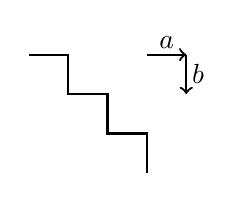
\begin{tikzpicture}[scale=0.5]

	% Staircase
	\draw[thick] (0,0) -- (1,0) -- (1,-1) -- (2,-1) -- (2,-2) -- (3,-2) -- (3,-3);
	
	% Elements
	\draw[thick,->] (3,0) -- (4,0); \node at (3.5,0.3) {$a$};
	\draw[thick,->] (4,0) -- (4,-1); \node at (4.3,-0.5) {$b$};
	
\end{tikzpicture} \\
	Example: staircase and the used elements $a$ and $b$
\end{center}
\vfill
\columnbreak
\begin{align*}
& 1) && \text{start} && S \rightarrow aA\\
& 2) && \text{repeat 1)} &&  A \rightarrow bS \\
& 3) && \text{end} &&  A \rightarrow b \\
\end{align*}
\end{multicols}
Now any staircase made up of $a$s and $b$ can be described by repeating these rules. 
E.g. $(1,3)$ is a staircase $a,b$. $(1,2,1,3)$ is $a,b,a,b$ , $\ldots$. \\

\paragraph{Directed line segments} The idea is, that section of an image are described by directed line segments

\begin{itemize}
\item There needs to be a set of
operations acting on the
primitives, such that a region or a
boundary can be described
\item The abstracted primitives need
some specific primitives, which
contain all directions
\item A shape can now be described as a string of operations.
\end{itemize}
\begin{figure}[h]
	\centering
	\begin{subfigure}[b]{0.45\textwidth}
		\centering
		\adjustbox{scale=0.6}{\begin{tikzpicture}
\draw[->, shorten >=4, shorten <= 4] (0,0) node [anchor=north] {Tail} -- (2,2) node [anchor=south] {Head};
\draw (0,0) node [circ] {};
\draw (2,2) node [circ] {};

\draw[->, shorten >=4, shorten <= 4] (3.5,-0.5) node [anchor=north] {Tail} -- (4,2) node [anchor=south] {Head};
\draw (3.5,-0.5) node [circ] {};
\draw (4,2) node [circ] {};

\draw  plot[smooth, tension=.7] coordinates {(-0.4,0.7) (0.2,1.7) (2.9,2.7) (2.1,0.6) (0.6,-0.6) (-0.3,-0.5) (-0.4,0.7)};

\draw  plot[smooth, tension=.7] coordinates {(3,-0.5) (3.3,0.7) (3.3,2.1) (3.8,3) (4.7,2.2) (4.6,1.2) (4.2,0.5) (4.3,-0.5) (4,-1.3) (3,-1.1) (3,-0.5)};
\end{tikzpicture}}
		\caption{Abstracted Primitives}
	\end{subfigure}
	\begin{subfigure}[b]{0.45\textwidth}
		\centering
		\adjustbox{scale=0.8}{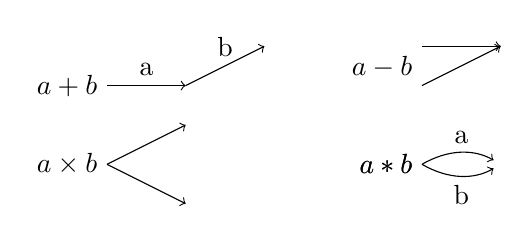
\begin{tikzpicture}[->]
\draw (0,0) node [anchor=east] {$a+b$} to node[anchor=south] {a} (1,0);
\draw (1,0) to node[anchor=south] {b} (2,0.5);

\draw (4,0.5) node [anchor=north east] {$a-b$} to (5,0.5);
\draw (4,0) to (5,0.5);

\draw (0,-1) node [anchor=east] {$a\times b$} to (1,-0.5);
\draw (0,-1) to (1,-1.5);

\draw[shorten >= 3] (4,-1) node [anchor=east] {$a*b$} to [bend left] node[anchor=south] {a} (5,-1);
\draw[shorten >= 3] (4,-1) node [anchor=east] {$a*b$} to [bend right] node[anchor=north] {b} (5,-1);
\end{tikzpicture}}
		\caption{Operations among primitives}
	\end{subfigure}
	\caption{Primitives}
\end{figure}

\paragraph{Tree descriptors} 
Information describing the meaning of a node and relating it to its neighbors can be stored in trees.
A texture may some times not be connected, then it can be described by trees. \\

Each tree has a unique node called the root $\$$ and is made up of subtrees. All leaves of a tree are called the frontier of the tree.

\begin{figure}[h]
	\centering
	\begin{subfigure}[b]{0.45\textwidth}
		\centering
		\adjustbox{scale=0.6}{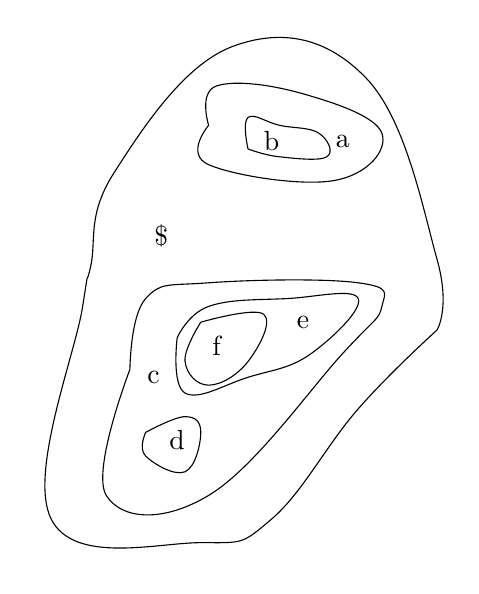
\begin{tikzpicture}

\draw  plot[smooth, tension=.7] coordinates {(0.3,0.5) (-0.7,-0.5) (-1.8,-1.9) (-2.7,-2.2) (-4.6,-1.9) (-4.2,0.8) (-4.1,1.3) (-3.8,2.5) (-2.3,4.1) (-0.6,3.7) (0.3,1.4) (0.3,0.5)};
\draw  plot[smooth, tension=.7] coordinates {(-2.7,0.6) (-2.9,0.1) (-2.6,-0.2) (-2.1,0.1) (-1.9,0.7) (-2.7,0.6)         };
\draw  plot[smooth, tension=.7] coordinates {(-3,0.4) (-2.6,0.8) (-1.6,0.9) (-0.7,0.9) (-1.3,0.2) (-2.1,-0.1) (-2.9,-0.3) (-3,0.4)};
\draw  plot[smooth, tension=.7] coordinates {(-3.6,0) (-3.4,0.9) (-2.6,1.1) (-0.7,1.1) (-0.4,0.8) (-0.9,0.2) (-2.6,-1.6) (-3.9,-1.6) (-3.6,0)};
\draw  plot[smooth, tension=.7] coordinates {(-3.4,-0.8) (-2.9,-0.6) (-2.7,-0.8) (-2.9,-1.3) (-3.4,-1.1) (-3.4,-0.8)};

\node at (-2.5,0.3) {f};
\node at (-1.4,0.6) {e};
\node at (-3,-0.9) {d};
\node at (-3.3,-0.1) {c};
\node at (-3.2,1.7) {$\$$};
\draw  plot[smooth, tension=.7] coordinates {(-2.1,2.8) (-2.1,3.2) (-1.7,3.1) (-1.2,3) (-1.1,2.7) (-1.7,2.7) (-2.1,2.8)};
\draw  plot[smooth, tension=.7] coordinates {(-2.6,3.1) (-2.5,3.6) (-1.4,3.5) (-0.4,3) (-1,2.4) (-2.6,2.6) (-2.6,3.1)};
\node at (-1.8,2.9) {b};
\node at (-0.9,2.9) {a};
\end{tikzpicture}}
		\caption{Simple composite region}
	\end{subfigure}
	\begin{subfigure}[b]{0.45\textwidth}
		\centering
		\adjustbox{scale=0.8}{\begin{tikzpicture}
\node {$\$$}
	child {node {a}
		child {node {b}}
	}
	child {node {c}
		child {node {d}}
		child {node {e}
			child {node {f}}
		}
	}
; 
\end{tikzpicture}}
		\caption{Tree representation}
	\end{subfigure}
	\caption{Tree descriptors}
\end{figure}
